\chapter{Methodology}
\label{chp:methodology}

\par This chapter discusses the methodology used to measure the effectiveness of \ac{ARG} at correctly classifying invalid and valid traffic, the maximum supportable hop rate at various network latencies, the maximum packet rate \ac{ARG} can handle, and the overall stability of the system under test. Section \ref{sec:problem_def} discusses the problem this research seeks to answer. Section \ref{sec:boundaries} defines the \ac{SUT} and Section \ref{sec:services} goes into detail on the possible outcomes of the \ac{CUT}. Section \ref{sec:workload} covers the workload presented to the \ac{SUT}, Section \ref{sec:metrics} covers the metrics collected, and Section \ref{sec:parameters} covers the configurable parameters of the \ac{SUT}. Section \ref{sec:factors} brings the previous sections together, giving a comprehensive list of the factors varied for each test. Section \ref{sec:exp_design} details the actual tests and the purpose of each.

\section{Problem Definition}
\label{sec:problem_def}
\subsection{Goals and Hypothesis}
\label{sec:goals}
\par This research seeks to test whether network address space randomization is suitable for deployment on a military network, as discussed in the previous chapter. Tests against this system are designed to answer four basic questions:

\begin{enumerate}
\item Does \ac{ARG} classify traffic correctly? What percentage of false positives (valid packets blocked) and false negatives (invalid traffic allowed through) does it introduce?
\item What is the max packet rate and throughput \ac{ARG} can handle?
\item What is the max hop rate---the frequency with which \ac{ARG} changes \acp{IP}---that still allows for reliable communication? How does latency affect this?
\item Is \ac{ARG} stable when presented with corrupt, malformed, or replayed packets?
\end{enumerate}

%\par The software developed and tested here attempts to interfere minimally with the network, a critical requirement for the real-world deployment of such technology. Systems \ac{ARG} touches---both inside and outside the ``protected'' networks---do not need any modifications to continue to function. The research done here provides data on whether this is true as a side effect, potentially valuable information for an organization considering employing a \ac{DYNAT} solution. However, validation of this design goal is not a primary objective. 

%\par The working hypothesis for this research is, as speculated by Sandia, a \ac{DYNAT} system allows for quick identification of unexpected (and potentially malicious) packets entering a network. There are few identifiers within the scope of \ac{DYNAT} by which outgoing packets could be filtered. Given that, no filtering is done for outbound packets and hence no change in behavior is observed when compared to the control network. 

\par It is hypothesized that \ac{ARG} correctly classifies 99\% of traffic it encounters when operating with a hop rate appropriate for the network latency. In addition, this thesis hypothesizes that packet loss become acceptable when the hop rate matches or exceeds the network latency, where acceptable loss is defined as less than 2\% \tbd{2\% figure from MIT wifi? Trying to find source... it's on an article about TCP-NC, but not in the actual paper.}. The other two questions under test are informational in nature as the results apply only to the specific implementation under test, but it is believed that \ac{ARG} is stable in the face of malformed traffic and it can handle at least 10 \ac{Mbps} of traffic. 

\subsection{Approach}
\label{sec:approach}
\par This research is done on a test network with nodes representing the types of hosts found on a typical, corporate-style network. These include trusted hosts inside trusted networks which communicate freely, internal and external servers that must be accessible to hosts inside these trusted networks, and malicious hosts outside the networks. A configurable custom hopping gateway sits in front of the trusted networks. 

\par Traffic generators and collectors run on this network, determining which traffic flows successfully make it to their destination. This includes examining both false positive and false negative rates, determining why \ac{ARG} rejects packets that should get through and why it allows packets that should be rejected. After a given test, logs and traffic captures are collated to form a complete picture of the traffic on the network before determining statistics.

\FloatBarrier
\section{System Boundaries}
\label{sec:boundaries}
\par The \ac{SUT} is \ac{ARG}, the custom \ac{IP} hopping gateway developed specifically for this effort. The basic components of this system, the various inputs into the system, possible outputs, and the metrics provided are illustrated in Figure \ref{fig:sut}. The sections following cover aspects of this diagram in more detail, with Section \ref{sec:services} discussing the possible outcomes, Section \ref{sec:workload} covering the workload, Section \ref{sec:parameters} detailing the parameters in use, and Section \ref{sec:metrics} covering the metrics collected.

\begin{figure}
	\caption{Address Routing Gateway}
	\label{fig:sut}
	\centering
	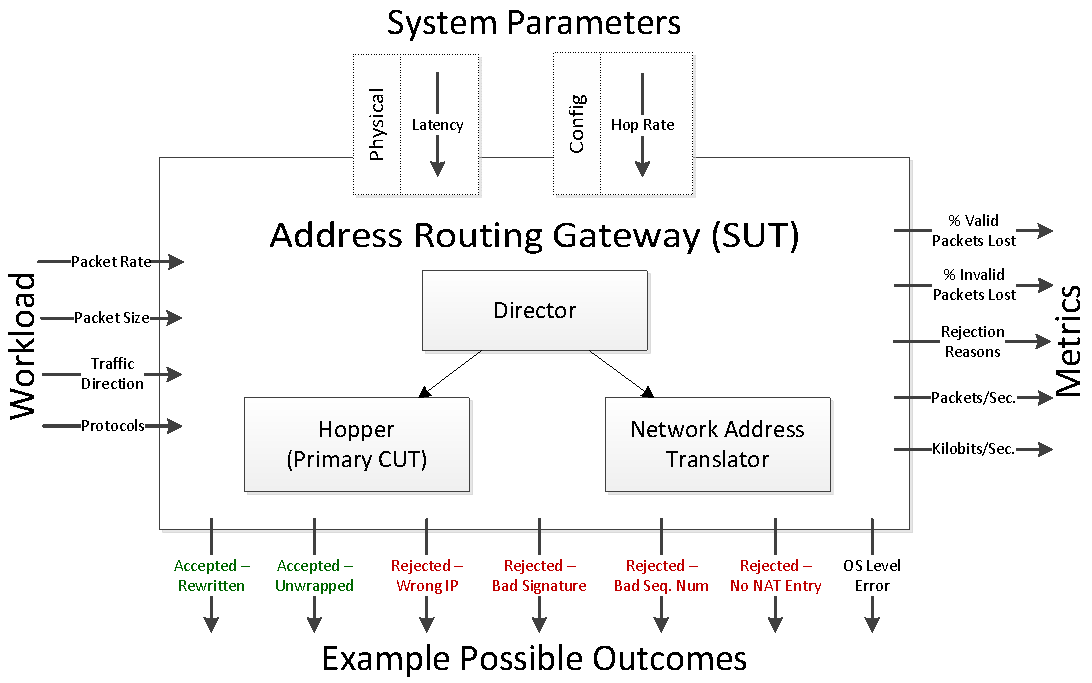
\includegraphics[width=1\textwidth]{sut}
\end{figure}

\FloatBarrier
\section{System Services}
\label{sec:services}
\par \ac{ARG} has three components that this thesis tests. Most important is the hopper module, which provides a rapidly-changing external \ac{IP} address and details on connected ARG networks. Using this information, it transports packets between ARG-protected networks. Packets to and from external hosts---hosts that are not part of an ARG network---go through the \ac{NAT} module. Finally, the director module hands packets off to each of the other modules and collects the results back to be logged and potentially acted upon. More details on these components are in Chapter \ref{chp:implementation}.

\par The potential outcomes of the director are shown below, broken into separate sections based on incoming or outgoing packets. Other services do not directly offer outcomes relevant to this research.

\begin{itemize}
\item Director - Incoming
	\begin{itemize}
	\item Rewritten and forwarded - Packet is from non-\ac{ARG} network and is rewritten via \ac{NAT} table before forwarding.
	\item Unwrapped and forwarded - Packet is from \ac{ARG} network and passes validation checks. Contents are extracted and forwarded internally.

	\item Incorrect source \ac{IP} - Packet is coming from an \ac{ARG} network but does not have the what the local gateway believes is the current source IP for the other gateway.
	\item Incorrect destination \ac{IP} - Packet is coming from an \ac{ARG} network but does not have the current local gateway \ac{IP} as the destination.
	\item Incorrect message size - The message length does not match the message type.
	\item Incorrect sequence number - The message's sequence number is not monotonically increasing. 
	\item Unable to verify signature/\ac{HMAC} - Packet signature invalid/nonexistent (if coming from an \ac{ARG} network).
	\item No \ac{NAT} bucket/entry - Packet is coming from a non-\ac{ARG} network but does not have a valid entry in the \ac{NAT} table.

	\item Misc - Some operating system-level errors may occur, resulting in rare errors in sending or receiving packets.
	\end{itemize}

\item Director - Outgoing
	\begin{itemize}
	\item Rewritten and forwarded - Packet is destined for non-\ac{ARG} network. An entry is made/retrieved from the \ac{NAT} table and used to rewrite packet.

	\item Gateway not connected - Packet was intended for an ARG network the gateway is aware of but not yet connected to.
	\item Wrapped and forwarded - Packet is destined for an \ac{ARG} network. Wrapped and placed on the external network.

	\item Misc - Some operating system-level errors may occur, resulting in rare errors in sending or receiving packets.
	\end{itemize}
\end{itemize}

\section{Workload}
\label{sec:workload}
\par Workload to the system is the traffic flowing through the \ac{ARG} gateways. Standard network traffic parameters like packet rate, packet size, number of simultaneous ongoing connections, and lifetime of connections play a role. However, it is important to note that the network performance itself is not a large concern of this research. Packet rate, for example, does provide useful information about the performance of \ac{ARG} itself, but the numbers apply only to this specific implementation. \ac{ARG}'s development does not focus on performance in this first iteration, so there are many possible areas for improvement. Previous research has shown that similar solutions have minimal impact on performance \cite{NAH}. 

\par Two parameters are more specific to \ac{ARG}. First, the proportion of traffic between protected networks verses traffic to external hosts varies the validation methods \ac{ARG} uses for each packet. Traffic flows that focus on connections between protected networks rely on current \ac{IP} synchronization and signatures, while traffic that originates externally exercises the \ac{NAT} table.

\par Second, the proportion of valid and invalid traffic---traffic that should or should not be permitted through \ac{ARG}---is a workload parameter. The reasons behind each packet's invalidity is also important: most of the possible outcomes from \ac{ARG} depend on \textit{why} a packet is invalid. The possible failure points here are incorrect external \acp{IP}, invalid packet signatures, and no entry in the \ac{NAT} table.

\section{Performance Metrics}
\label{sec:metrics}
\par As previously stated, this research is primarily focused on the classification accuracy of \ac{ARG} and the interaction of hop rate and latency. Measurements on \ac{ARG} therefore focus on the outcomes from the Director. However, basic statistics on network performance are collected. The metrics of interest include:

\begin{itemize}
\item Percentage of invalid packets accepted
	\par If a packet that should have been rejected is accepted by \ac{ARG}, it is possible for an attacker to sneak into the network regardless of the \ac{DYNAT}'s existence. This then is the true measure of whether or not \ac{ARG} is protecting the network. If it functions correctly, this number should remain at zero for all experiments with \ac{ARG} enabled.

\item Percentage of valid packets rejected
	\par In ideal circumstances, this will also be zero. However, network conditions may result in failures here, which on a real-world network might result in a disruption of service. 

\item Number of each type of rejection (each possible outcome from the director)
	\par This reveals where in the processing stage packets are typically caught. If packets get caught in the later stages of validation---e.g., signature checking---then processing time has been wasted.

\item Packets per second and \acf{Kbps}
	\par An easy check on \ac{ARG}'s performance is comparing the amount of traffic it is handling against the loss rate it shows. Information about both the number of packets and the raw number of bits it processes may reveal slightly different results, so collecting both is important.
\end{itemize}

\section{System Parameters}
\label{sec:parameters}
\par As a network application, \ac{ARG} is affected by both the machine on which it runs and the network over which it communicates. \ac{ARG}'s local performance is most affected by processor and memory speeds, with encryption potentially consuming a fair amount of processor time and memory speeds impacting virtually all aspects of operation.

\par The primary physical network parameter that affects \ac{ARG} is latency. To ensure that two \ac{ARG} gateways are able to communicate reliably, packets sent from one gateway to the other must arrive before the \ac{IP} address used in the send are no longer current. If hops occur too frequently then a high one-way latency will cause sent packets to frequently arrive after the receiving gateway has hopped to a different \ac{IP} address. 

\par The primary configuration setting for \ac{ARG} is the hop rate. \ac{ARG} allows the time between hops to be customized from several times a second to minutes apart with millisecond precision. Each gateway may be configured to hop at different rates, but for the sake of this thesis the hop rates are always identical in a given test.

\section{Factors}
\FloatBarrier
\label{sec:factors}
\par Based on the system and workload parameters given above, the following factors are varied as part of the experiment. All others remain constant throughout the experiment. Factors and levels are summarized in Table \ref{tbl:factors} and described in detail below.

\begin{table}
\begin{center}
	\caption{Factors and Levels}
	\label{tbl:factors}
	
	\begin{tabular}{r|l}
	\textbf{Factor} & \textbf{Possible Levels } \\
	\hline
	Hop rate (ms) & 1000, 500, 300, 200, 100, 75, 60, 50, 40, 30, 15, 10, 5\\
	Latency (ms) & 500, 100, 30, 20, 0\\
	Packet Delay (s) & 0.3, 0.2, 0.1, 0.05, 0.01, 0.005, 0.001\\
	Traffic direction and type & See detailed description
	\end{tabular}
\end{center}
\end{table}

\begin{itemize}
\item Hop rate
	\par Varying the rate at which \ac{ARG} switches to a new external \ac{IP} allows testing of the maximum supportable hop rate. Hops every 1000 milliseconds give ample time for packets to travel across the network at all but the most extreme latencies, while hops every 5 milliseconds stress even ideal network conditions.

\item Latency between \ac{ARG} gateways
	\par The test network runs through a single switch running four \acp{VLAN}, with an average latency under 1 millisecond. Introducing artificial latency simulates a more realistic range of environments.

\item Packet Delay
	\par Each test spawns a number of traffic generators at different points in the test network. The packet delay shown here is used as a wait between each packet sent. Lower delays result in more frequent sends and force the gateways to deal with more packets per second.

\item Traffic direction and type
	\par \ac{ARG} is designed to handle \ac{TCP}, \ac{UDP}, and \ac{ICMP} traffic. All tests use equal amounts of \ac{TCP} and \ac{UDP} traffic, but some vary the direction. Section \ref{sec:exp_design} gives a full description of the various tests and Figure \ref{fig:testnum_flows} illustrates the direction of all traffic on the network.
\end{itemize}

\section{Evaluation Technique}
\label{sec:eval_technique}
\par Measurement is used to obtain results for each factor level. Due to the fairly complex interactions needed between \ac{ARG} gateways and the processing needed to decide how to handle packets, simulating the system would likely require an equal amount of work with little benefit.

\par Setup of the test environment involves a basic 7-node network: three gateways running \ac{ARG}, one system on the network protected by each gateway, and one host outside the network. Figure \ref{fig:argnetwork} shows the network and the names given to the various systems.

\begin{figure}
	\centering
	\caption{ARG Network Layout Overview}
	\label{fig:argnetwork}
	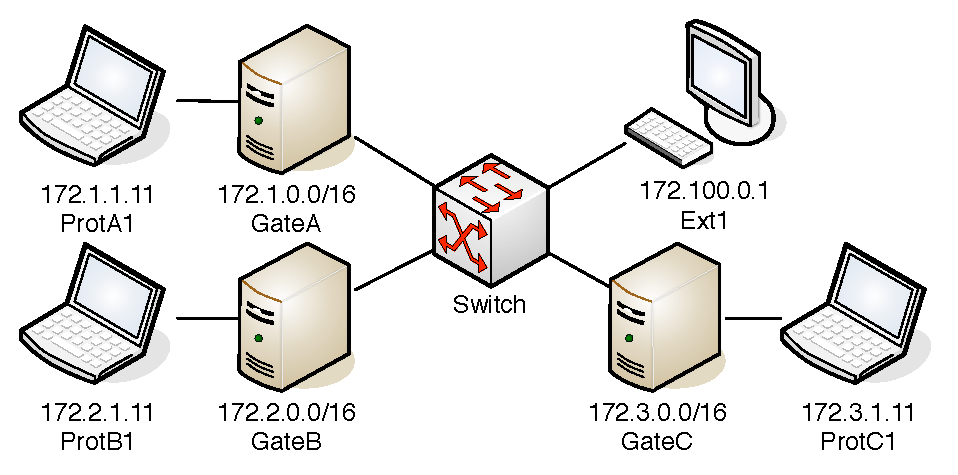
\includegraphics[width=0.75\textwidth]{thesis_network}
\end{figure}

\par Protected clients behind the gateways (\texttt{ProtA1}, \texttt{ProtB1}, and \texttt{ProtC1}) may communicate freely. The protected clients may also talk out to the external host (\texttt{Ext1}), and the external hosts must then---once that connection is established---be able to talk back into the network. There is additional administrative traffic directly between the gateways (\texttt{GateA}, \texttt{GateB}, and \texttt{GateC}). These three basic traffic flows are ``valid'' traffic.

\par All traffic beyond what is described above is ``invalid.'' For example, \texttt{Ext1} is not allowed to send traffic in to the protected clients or the gateways without them first initiating the connection. Malformed traffic sent by any host is also considered invalid. In either case, invalid traffic should be stopped at the earliest possible opportunity (i.e., the gateway rejects the packet and keeps it from reaching the internal host) and the system must remain stable.

\par To collect data, each system runs the traffic collection program \texttt{tcpdump} to capture the traffic sent and received into \ac{PCAP} files. Traffic generators are then spawned as appropriate on each system in the network, each of which logs their sends and receives. After a given trial, the \ac{PCAP} files and traffic generator logs are collated and processed with custom scripts to determine the metrics described in Section \ref{sec:metrics}. More details on the traffic generators and test run sequence can be found in Appendixes \ref{chp:testseq} and \ref{chp:generators}.

\par All trials run on physical network of seven servers. Each server runs Ubuntu 12.04.1 Server Edition with four gigabytes of \ac{RAM} and a \tbd{CPU} gigahertz quad-core Intel Xeon. A single switch with four \acp{VLAN} connects each system at 100 \ac{Mbps}.

\section{Experimental Design}
\label{sec:exp_design}
\par Based on the factors given in Section \ref{sec:factors} and the goals of this research (as laid out in Section \ref{sec:goals}), there are eight traffic flows of interest. Each consists of different types of traffic and flow destinations. These are most easily visualized in Figure \ref{fig:testnum_flows}.

\begin{figure}
\caption[Experiment Traffic Flows]{Experiment Traffic Flows. Black is valid traffic, red is invalid. \tbd{Perhaps make two wide.}}
\label{fig:testnum_flows}
\centering
\begin{subfigure}[b]{0.328\linewidth}
	\centering
	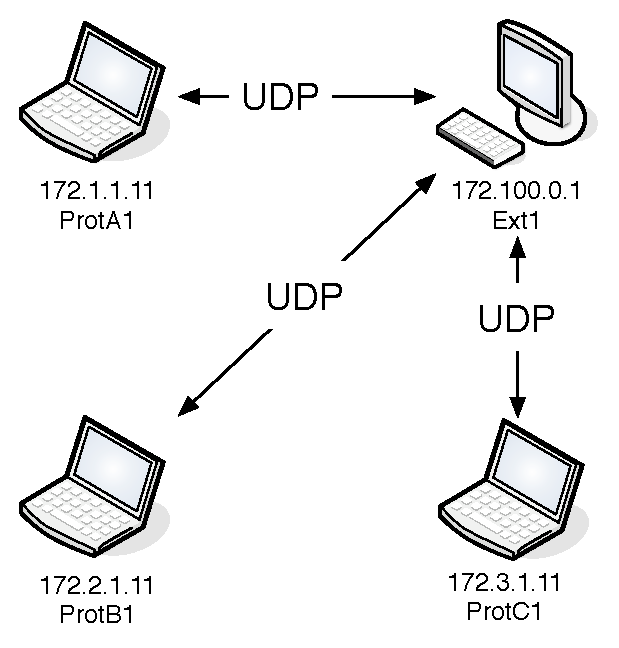
\includegraphics[width=1.0\linewidth]{test_traffic_0}
	\caption{Test 0}
\end{subfigure}
\begin{subfigure}[b]{0.328\linewidth}
	\centering
	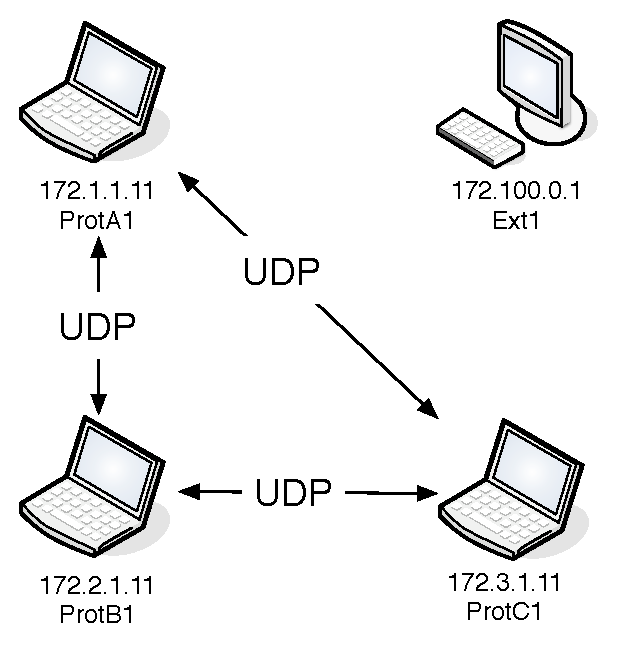
\includegraphics[width=1.0\linewidth]{test_traffic_1}
	\caption{Test 1}
\end{subfigure}
\begin{subfigure}[b]{0.328\linewidth}
	\centering
	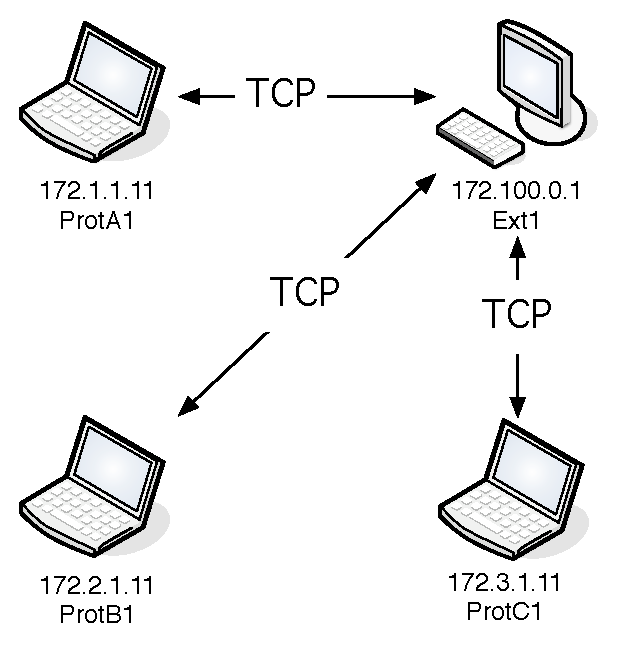
\includegraphics[width=1.0\linewidth]{test_traffic_2}
	\caption{Test 2}
\end{subfigure}
\begin{subfigure}[b]{0.328\linewidth}
	\centering
	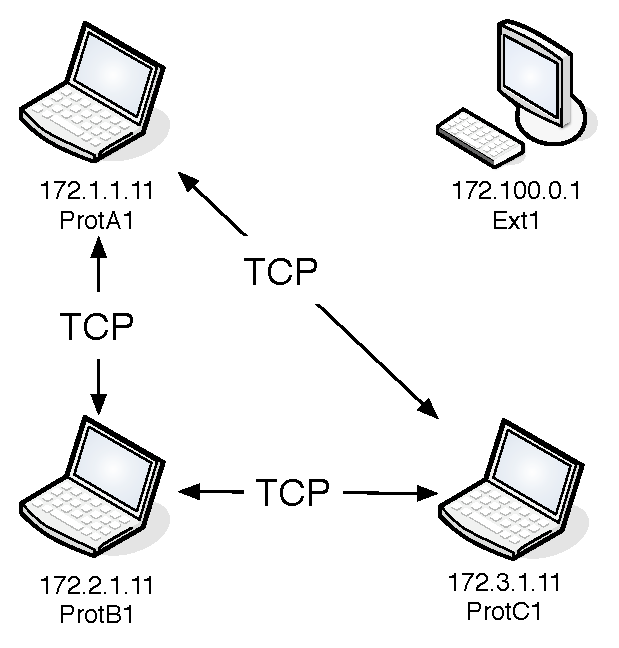
\includegraphics[width=1.0\linewidth]{test_traffic_3}
	\caption{Test 3}
\end{subfigure}
\begin{subfigure}[b]{0.328\linewidth}
	\centering
	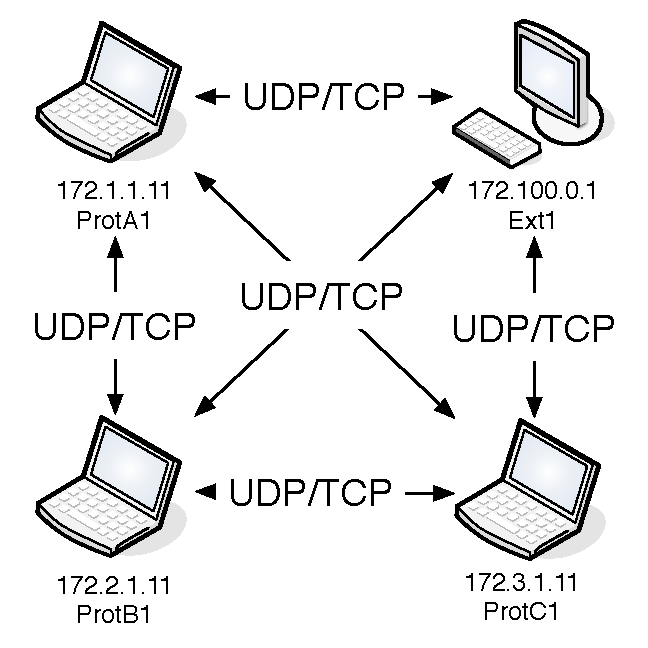
\includegraphics[width=1.0\linewidth]{test_traffic_4}
	\caption{Test 4}
\end{subfigure}
\begin{subfigure}[b]{0.328\linewidth}
	\centering
	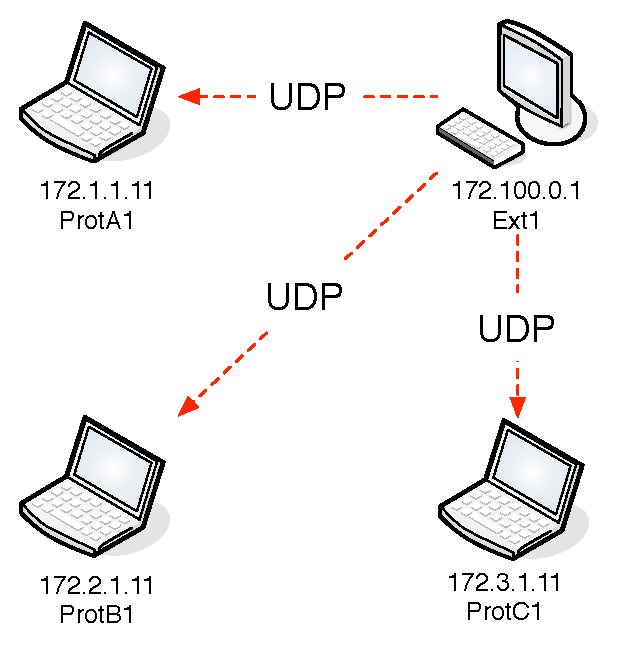
\includegraphics[width=1.0\linewidth]{test_traffic_5}
	\caption{Test 5}
\end{subfigure}
\begin{subfigure}[b]{0.328\linewidth}
	\centering
	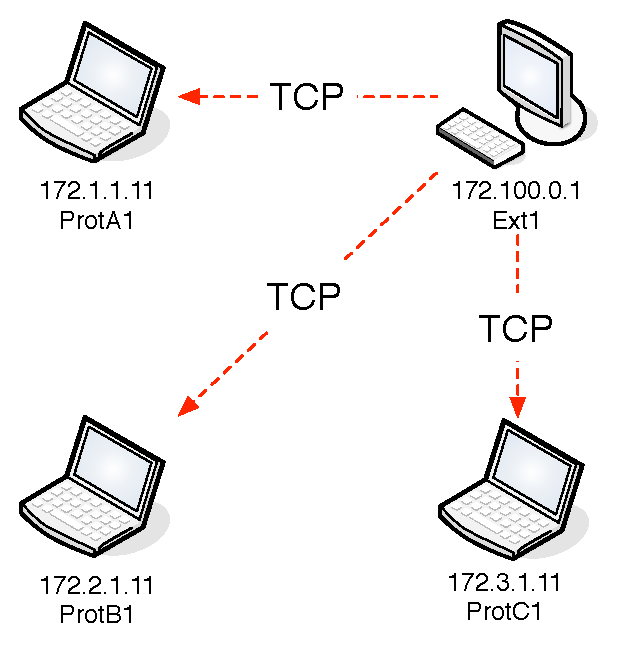
\includegraphics[width=1.0\linewidth]{test_traffic_6}
	\caption{Test 6}
\end{subfigure}
\begin{subfigure}[b]{0.328\linewidth}
	\centering
	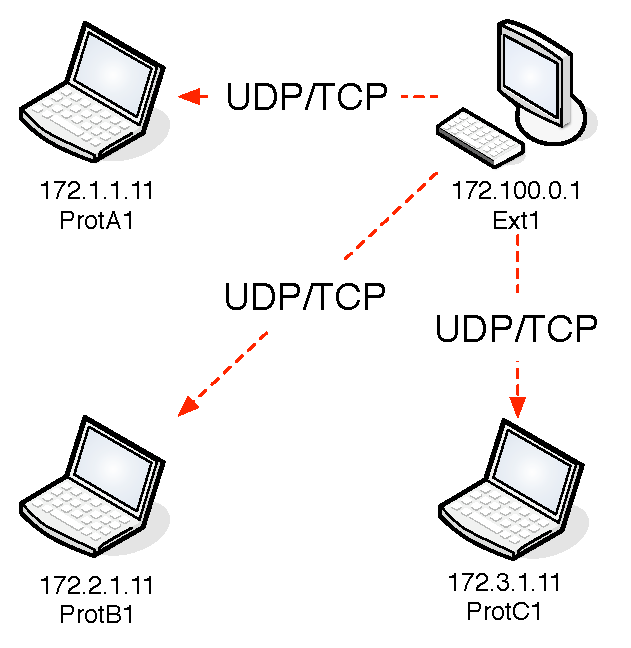
\includegraphics[width=1.0\linewidth]{test_traffic_7}
	\caption{Test 7}
\end{subfigure}
\begin{subfigure}[b]{0.328\linewidth}
	\centering
	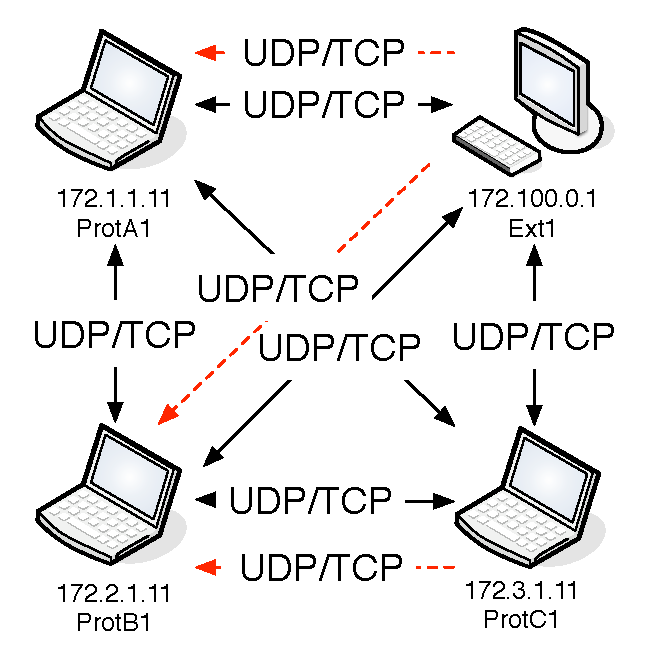
\includegraphics[width=1.0\linewidth]{test_traffic_8}
	\caption{Test 8}
\end{subfigure}
\end{figure}

\par These possible traffic flows are used in four sets of experiments, given below. Each experiment set answers a different research goal.
\begin{itemize}
	\item Basic tests
	\par This sequence of tests verifies that \ac{ARG} classifies traffic correctly by running every test shown in Figure \ref{fig:testnum_flows} against \ac{ARG}. Latency is set to 20 milliseconds for all tests and traffic generators produce packets around every 0.3 seconds (actual traffic rate is higher due to responses and \ac{TCP} acknowledgment packets). To determine if hop rate has an large impact on certain types of traffic, every test runs twice, once with a slow hop rate (500 ms) and one close to double the latency (50 ms).

	\item Max Throughput
	\par This sequence gives an indication of what throughput and packet rate \ac{ARG} is capable of handling. Packet delay goes through all levels shown in Table \ref{tbl:factors}, which leads to roughly corresponding increases in the throughput the gateways must handle. Hop rate changes between 500 ms and 50 ms to see if the additional \ac{IP} calculation load impacts the maximum rate. Test 4 is used in all runs to exercise all possible valid traffic flows. Latency is set to 20 ms.

	\item Max hop rate
	\par This sequence determines the maximum hopping rate at various latencies. Hop rate and latency go through the levels shown in Table \ref{tbl:factors} in a full factorial fashion (every latency-hop rate combination). Packet rate is fixed at 0.3 seconds and Test 4 is used throughout.

	\item Fuzzer
	\par This sequence is not tested rigorously for traffic flow success and failure, but ensures that \ac{ARG} remains stable despite malformed traffic. Test 8 is used, with the addition of fuzzers on each gateway that replay and/or alter traffic they see. Hop rate varies between 500 ms and 50 ms, latency is fixed at 20 ms, and packets are sent at 0.3 second intervals.
\end{itemize}

\par A 95\% confidence interval is used for all experiments. Experiments are each run for five minutes, sufficient time for the system to stabilize (pilot studies show that \ac{ARG} fully connects in under 10 seconds on the test network). Wide variation is possible in the actual traffic seen in a single run, so a minimum of 10 replications are used for each experiment.

\section{Summary}
\label{sec:method_summary}
\par This chapter discusses the methodology and goals of this research. It then defines the \ac{SUT} and its relevant factors. Finally, the test network setup and the exact tests run against it are covered, along with what metrics are collected and analyzed. 

